% ============================================================
% HIGH-PERFORMANCE CREDIT RISK ASSESSMENT
% SIMD-Accelerated C++ MLP for Low-Latency Default Prediction
% Beamer deck - same visual design as the drowsiness-detector deck
% ============================================================

\documentclass[aspectratio=169]{beamer}

\usetheme{Madrid}
\usecolortheme{default}

\definecolor{primary}{RGB}{0, 33, 71} % Oxford Blue
\definecolor{accent}{RGB}{220, 50, 50}
\definecolor{lightgray}{RGB}{245, 245, 245}
\definecolor{mlgreen}{RGB}{34, 139, 34}

\setbeamercolor{structure}{fg=primary}
\setbeamercolor{alerted text}{fg=accent}
\setbeamercolor{normal text}{fg=black!85!primary}
\setbeamercolor{block title}{bg=primary!9, fg=primary}
\setbeamercolor{block title alerted}{bg=accent!11, fg=accent!90!black}
\setbeamercolor{block body}{bg=primary!3}
\setbeamercolor{block body alerted}{bg=accent!4}
\setbeamercolor{palette primary}{bg=primary, fg=white}
\setbeamercolor{palette secondary}{bg=primary, fg=white}
\setbeamercolor{palette tertiary}{bg=primary, fg=white}
\setbeamercolor{palette quaternary}{bg=primary, fg=white}
\setbeamertemplate{blocks}[rounded][shadow=false]

\usepackage{helvet}
\renewcommand{\familydefault}{\sfdefault}
\usepackage{graphicx}
\usepackage{tikz}
\usetikzlibrary{shapes.geometric, arrows.meta, positioning, fit, backgrounds, calc}
\usepackage{booktabs}
\usepackage{array}
\usepackage{colortbl}
\usepackage{xcolor}
\usepackage{amsmath}
\usepackage{listings}
\usepackage{appendixnumberbeamer}
\newcommand{\cit}[1]{\textsuperscript{\textcolor{accent}{[#1]}}}
\lstdefinestyle{cpp}{language=C++, basicstyle=\ttfamily\fontsize{6.9}{8.3}\selectfont,
  keywordstyle=\color{primary}\bfseries, commentstyle=\color{mlgreen!80!black}\itshape,
  stringstyle=\color{accent}, showstringspaces=false, columns=fixed, keepspaces=true,
  backgroundcolor=\color{primary!4}, frame=single, rulecolor=\color{primary!25},
  framesep=3pt, xleftmargin=3pt, xrightmargin=3pt, aboveskip=0pt, belowskip=0pt,
  morekeywords={vector,string,mutable,override,size_t,float,int}}

\setbeamertemplate{navigation symbols}{}
\setbeamertemplate{itemize items}[circle]\setbeamercolor{itemize item}{fg=accent}
\setbeamerfont{block title}{size=\small}

% ---------- footer (same as source deck) ----------
\setbeamertemplate{footline}{%
  \vbox{\hbox to\paperwidth{\hskip6mm{\color{primary!55}\fontsize{6.5}{8}\selectfont\bfseries ARYA H. RAVAL\ \ $\cdot$\ \ 25EC415\ \ $\cdot$\ \ 204ES: OBJECT ORIENTED PROGRAMMING}\hfill
    {\color{primary!55}\fontsize{6.5}{8}\selectfont\bfseries\insertframenumber\,/\,\inserttotalframenumber}\hskip6mm}\vskip0.5mm
   {\color{primary}\rule{\dimexpr\paperwidth*\insertframenumber/\inserttotalframenumber\relax}{0.6mm}}\vskip-0.2mm}}

\title[Credit Risk MLP]{\textbf{High-Performance Credit Risk Assessment:}\\
\small SIMD-Accelerated C++ Multi-Layer Perceptron for Low-Latency Default Prediction}
\author{Arya H. Raval}
\institute{Birla Vishvakarma Mahavidyalaya}
\date{October 2026}

% ---------- TikZ styles (same as source deck) ----------
\tikzset{
  block/.style={rectangle, rounded corners=4pt, minimum width=2.2cm,
    minimum height=0.8cm, text centered, draw=primary, fill=lightgray,
    font=\small, text width=2.2cm},
  mlblock/.style={rectangle, rounded corners=4pt, minimum width=2.2cm,
    minimum height=0.8cm, text centered, draw=mlgreen, fill=mlgreen!10,
    font=\small\bfseries, text width=2.2cm},
  alertblock/.style={rectangle, rounded corners=4pt, minimum width=2.2cm,
    minimum height=0.8cm, text centered, draw=accent, fill=accent!10,
    font=\small, text width=2.2cm},
  arrow/.style={-{Stealth[length=4pt]}, thick, color=primary},
  mlarrow/.style={-{Stealth[length=4pt]}, thick, color=mlgreen},
  neuron/.style={circle, draw=primary, fill=white, minimum size=0.36cm, inner sep=0pt, font=\tiny},
  hneuron/.style={circle, draw=mlgreen, fill=mlgreen!12, minimum size=0.36cm, inner sep=0pt, font=\tiny},
  oneuron/.style={circle, draw=accent, fill=accent!12, minimum size=0.46cm, inner sep=0pt, font=\scriptsize},
}

\newcommand{\sigmoid}{\sigma}
\newcommand{\refitem}[2]{\par\noindent\hangindent=1.1cm\hangafter=1 \makebox[1.1cm][l]{[#1]}#2}

\newenvironment{eq}[1]{\begin{minipage}[t][#1][t]{\linewidth}\raggedright\hyphenpenalty=10000 }{\end{minipage}}
\begin{document}

% ============================================================
% 1. TITLE
% ============================================================
{
\setbeamertemplate{footline}{}
\begin{frame}[plain]
  \begin{columns}[c]
    \column{0.15\textwidth}
      \centering
      
\includegraphics[width=1.6cm]{Birla_Vishvakarma_Mahavidyalaya_logo.png}
    \column{0.70\textwidth}
      \centering
      {\small\textbf{Birla Vishvakarma Mahavidyalaya, Engineering College}}\\[0.05cm]
      {\footnotesize Department of Electronics \& Communication Engineering}\\[0.05cm]
      {\footnotesize Subject: \textbf{204ES: Object Oriented Programming}}
    \column{0.15\textwidth}
      \centering
      
\includegraphics[width=1.6cm]{fnewgtulogo.png}
  \end{columns}

  \vspace{0.25cm}
  {\color{accent}\hrule height 1.4pt}
  \vspace{0.3cm}

  \begin{center}
    {\large\textbf{\color{primary}High-Performance Credit Risk Assessment:}}\\[0.2cm]
    {\small SIMD-Accelerated C++ \textcolor{mlgreen}{\textbf{Multi-Layer Perceptron}}
      for Low-Latency Default Prediction}\\[0.1cm]
    {\footnotesize UCI Credit Card Default Dataset}
  \end{center}

  \vspace{0.3cm}
  {\color{accent}\hrule height 1.4pt}
  \vspace{0.45cm}

  \begin{columns}[c]
    \column{0.25\textwidth}\centering
      {\footnotesize\textbf{Student Name}}\\[0.1cm]
      {\footnotesize Arya H. Raval}
    \column{0.25\textwidth}\centering
      {\footnotesize\textbf{Student ID}}\\[0.1cm]
      {\footnotesize 25EC415}
    \column{0.25\textwidth}\centering
      {\footnotesize\textbf{Subject Code}}\\[0.1cm]
      {\footnotesize 204ES}
  \end{columns}
\end{frame}
}

% ============================================================
% 2. PROBLEM STATEMENT
% ============================================================
\begin{frame}{Problem Statement}
  \begin{columns}[T]
    \column{0.48\textwidth}
      \begin{block}{The Task}
\begin{eq}{4.2cm}
        \small
        Given an account's credit limit, demographics, six months of repayment
        status, bill amounts and payments, predict whether the client will
        \textbf{default next month}.
        \begin{itemize}
          \item Binary classification, \textbf{23 input features}
          \item \textbf{30,000} credit-card clients\cit{1,2}
          \item Only \textbf{22.1\%} of clients default
        \end{itemize}
      \end{eq}
      \end{block}
    \column{0.48\textwidth}
      \begin{alertblock}{The Challenge}
\begin{eq}{4.2cm}
        \small
        \begin{itemize}
          \item \textbf{Class imbalance:} predicting ``no default'' for everyone already
                scores \textbf{77.9\%} accuracy
          \item \textbf{Latency:} scoring must be fast and predictable when it
                sits inside a live decision loop
          \item \textbf{Overhead:} for a tiny model, framework call overhead can
                cost more than the maths
        \end{itemize}
      \end{eq}
      \end{alertblock}
  \end{columns}

  \vspace{0.05cm}
  \begin{center}
    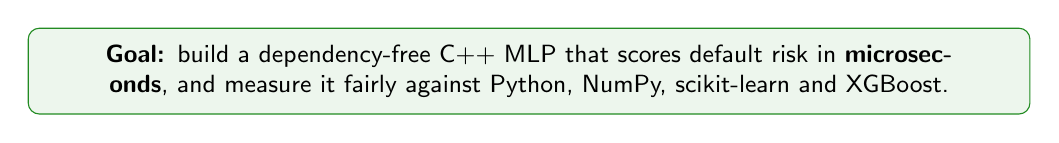
\begin{tikzpicture}
      \node[draw=mlgreen, fill=mlgreen!8, rounded corners=4pt, text width=12.3cm, align=center,
            inner sep=6pt, font=\small]
        {\textbf{Goal:} build a dependency-free C++ MLP that scores default risk in
         \textbf{microseconds}, and measure it fairly against Python, NumPy, scikit-learn and XGBoost.};
    \end{tikzpicture}
  \end{center}
\end{frame}

% ============================================================
% 3. MOTIVATION
% ============================================================
\begin{frame}{Motivation}
  \begin{columns}[T]
    \column{0.48\textwidth}
      \begin{alertblock}{Why credit risk?}
\begin{eq}{3.7cm}
        \small
        \begin{itemize}
          \item Lenders must decide limits, approvals and collections
                for \textbf{millions of accounts}
          \item A missed defaulter costs far more than a declined good customer,
                so scoring accuracy has a direct financial effect\cit{6}
          \item Portfolios are re-scored repeatedly: daily, and under stress scenarios
        \end{itemize}
      \end{eq}
      \end{alertblock}
    \column{0.48\textwidth}
      \begin{block}{Why hand-written C++?}
\begin{eq}{3.7cm}
        \small
        \begin{itemize}
          \item \textcolor{mlgreen}{\textbf{Latency:}} no interpreter, no garbage collector,
                no heap allocation in the hot loop
          \item \textcolor{mlgreen}{\textbf{Portability:}} 401 weights, standard library only
          \item \textcolor{mlgreen}{\textbf{Understanding:}} forward pass and backpropagation
                written out, not hidden in a framework
        \end{itemize}
      \end{eq}
      \end{block}
  \end{columns}

  \vspace{0.45cm}
  \centering
  \textit{``For a model this small, the speed question is about overhead, not arithmetic.''}
\end{frame}

% ============================================================
% 4. PROJECT ARCHITECTURE
% ============================================================
\begin{frame}{Project Architecture}
  \centering
  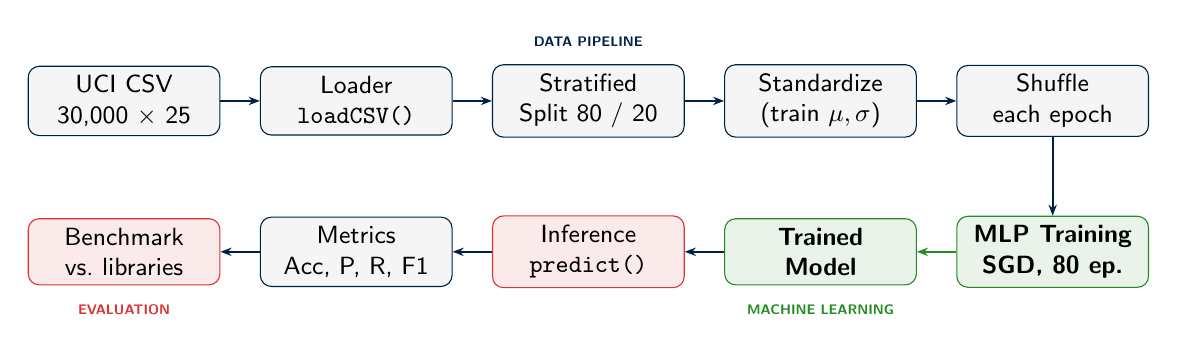
\begin{tikzpicture}[node distance=0.45cm and 0.5cm]
    \node[block]    (csv)   {UCI CSV\\30,000 $\times$ 25};
    \node[block,    right=of csv]   (load)  {Loader\\\texttt{loadCSV()}};
    \node[block,    right=of load]  (split) {Stratified\\Split 80 / 20};
    \node[block,    right=of split] (std)   {Standardize\\(train $\mu,\sigma$)};
    \node[block,    right=of std]   (shuf)  {Shuffle\\each epoch};

    \node[mlblock,  below=1.0cm of shuf]  (train) {MLP Training\\SGD, 80 ep.};
    \node[mlblock,  left=of train]        (model) {Trained\\Model};
    \node[alertblock, left=of model]      (infer) {Inference\\\texttt{predict()}};
    \node[block,    left=of infer]        (metr)  {Metrics\\Acc, P, R, F1};
    \node[alertblock, left=of metr]       (bench) {Benchmark\\vs.\ libraries};

    \draw[arrow] (csv)  -- (load);
    \draw[arrow] (load) -- (split);
    \draw[arrow] (split)-- (std);
    \draw[arrow] (std)  -- (shuf);
    \draw[arrow] (shuf) -- (train);
    \draw[mlarrow] (train) -- (model);
    \draw[arrow] (model) -- (infer);
    \draw[arrow] (infer) -- (metr);
    \draw[arrow] (metr)  -- (bench);

    \node[above=0.1cm of split, font=\tiny\bfseries, color=primary] {DATA PIPELINE};
    \node[below=0.12cm of model, font=\tiny\bfseries, color=mlgreen] {MACHINE LEARNING};
    \node[below=0.12cm of bench, font=\tiny\bfseries, color=accent] {EVALUATION};
  \end{tikzpicture}

  \vspace{0.25cm}
  {\footnotesize
    \textcolor{primary}{\rule{0.5cm}{4pt}}~Data processing\quad
    \textcolor{mlgreen}{\rule{0.5cm}{4pt}}~ML component\quad
    \textcolor{accent}{\rule{0.5cm}{4pt}}~Inference / evaluation}

  \vspace{0.2cm}
  {\footnotesize Single C++ file, \texttt{g++ -O3 -march=native}. Standardization uses
   \textbf{training statistics only}. \textbf{Fixed seed:} split, initial weights and shuffle orders are
   generated once and shared by every implementation, so results are reproducible.}
\end{frame}

% ============================================================
% 5. MODEL ARCHITECTURE
% ============================================================
\begin{frame}{Model Architecture: The MLP}
  \begin{columns}[c]
    \column{0.52\textwidth}
      \centering
      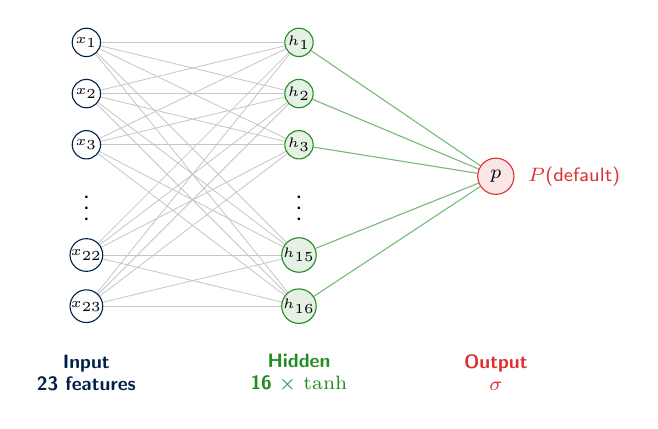
\begin{tikzpicture}[x=1cm,y=1cm]
        % input layer
        \foreach \i/\y/\l in {1/2.0/$x_1$, 2/1.35/$x_2$, 3/0.7/$x_3$, 4/-0.7/{\tiny$x_{22}$}, 5/-1.35/{\tiny$x_{23}$}} {
          \node[neuron] (in\i) at (0,\y) {\l};
        }
        % hidden layer
        \foreach \i/\y/\l in {1/2.0/$h_1$, 2/1.35/$h_2$, 3/0.7/$h_3$, 4/-0.7/{\tiny$h_{15}$}, 5/-1.35/{\tiny$h_{16}$}} {
          \node[hneuron] (h\i) at (2.7,\y) {\l};
        }
        \node[oneuron] (out) at (5.2,0.3) {$p$};
        \node[font=\scriptsize, color=accent, right=0.05cm of out] {$P$(default)};
        \begin{scope}[on background layer]
          \foreach \i in {1,...,5} {
            \foreach \j in {1,...,5} {
              \draw[gray!45, line width=0.3pt] (in\i) -- (h\j);
            }
            \draw[mlgreen!60, line width=0.4pt] (h\i) -- (out);
          }
        \end{scope}
        \node at (0,0) {$\vdots$};
        \node at (2.7,0) {$\vdots$};
        \node[font=\scriptsize\bfseries, color=primary, align=center] at (0,-2.2) {Input\\23 features};
        \node[font=\scriptsize\bfseries, color=mlgreen, align=center] at (2.7,-2.2) {Hidden\\16 $\times$ $\tanh$};
        \node[font=\scriptsize\bfseries, color=accent, align=center] at (5.2,-2.2) {Output\\$\sigma$};
      \end{tikzpicture}

    \column{0.46\textwidth}
      \begin{block}{Forward pass}
        \small
        \begin{align*}
          \mathbf{h} &= \tanh(W_1\mathbf{x} + \mathbf{b}_1) \\
          p &= \sigma(\mathbf{w}_2^{\top}\mathbf{h} + b_2), \quad \sigma(z)=\tfrac{1}{1+e^{-z}}
        \end{align*}
      \end{block}
      \begin{block}{Size and setup}
        \footnotesize
        \begin{itemize}
          \item Parameters: $23{\cdot}16 + 16 + 16 + 1 = \mathbf{401}$ (about 1.6\,KB in \texttt{float})
          \item Init: $\mathcal{N}(0,\,2/n_{\text{in}})$ (He-style)\cit{5}
          \item Loss: binary cross-entropy
          \item Optimizer: per-sample SGD\cit{3,4}, $\eta = 0.01$
          \item Decision: predict default if $p \geq 0.5$
        \end{itemize}
      \end{block}
  \end{columns}
\end{frame}

% ============================================================
% 6. FURTHER EXPLANATION
% ============================================================
\begin{frame}{How It Works, End to End}
  \begin{columns}[T]
    \column{0.485\textwidth}
      \begin{block}{\small 1. Prepare the data}
        \footnotesize
        Keep 23 features and the label. \textbf{Stratified} 80/20 split (22\% defaults in both), then standardize with \textbf{training} statistics only\cit{4} (no test-set leakage):
        \[ x' = \frac{x-\mu_{\text{train}}}{\sigma_{\text{train}}} \]
      \end{block}
      \begin{block}{\small 2. Learn (per client, 80 epochs)}
        \footnotesize
        Guess, compare with the true label $y$, and nudge every weight against its error (backpropagation\cit{3}):
        \[ dz = p - y, \qquad W \leftarrow W - \eta\,\frac{\partial L}{\partial W},\quad \eta=0.01 \]
      \end{block}
    \column{0.485\textwidth}
      \begin{block}{\small 3. Predict}
        \footnotesize
        The same forward pass gives a default probability; flag the client if it passes the threshold:
        \[ p = \sigma\!\big(\mathbf{w}_2^{\top}\tanh(W_1\mathbf{x}+\mathbf{b}_1)+b_2\big),\quad \hat{y}=\mathbf{1}[p\ge 0.5] \]
      \end{block}
      \begin{block}{\small 4. Check on the held-out 20\%}
        \footnotesize
        Count hits and misses:
        \[ P=\tfrac{TP}{TP+FP},\quad R=\tfrac{TP}{TP+FN},\quad F_1=\tfrac{2PR}{P+R} \]
      \end{block}
  \end{columns}
  \vspace{0.15cm}
  \centering\small\textcolor{mlgreen}{\textbf{Why it is fast:}} a tiny model with no framework around it, so almost no overhead surrounds the arithmetic.
\end{frame}

% ============================================================
% 6b. OOP CONCEPTS USED
% ============================================================
\begin{frame}{OOP Concepts Used in This Project}
  \begin{columns}[T]
    \column{0.49\textwidth}
      \begin{block}{\small Designing the classes}
\begin{eq}{4.35cm}
        \scriptsize
        \begin{itemize}
          \item \textbf{Class and object:} \texttt{class FastMLP} holds the weights and the behaviour; \texttt{FastMLP net(23,16)} is the trained model
          \item \textbf{Encapsulation:} weights, biases and buffers are \texttt{private}; outside code only calls \texttt{predict()} and \texttt{trainOne()}
          \item \textbf{Constructor and init list:} sizes the arrays, seeds the RNG and draws the He-initial weights, so the object is never half-built
          \item \textbf{Structs as data types:} \texttt{Sample} (features + label) and \texttt{Metrics} (counters + \texttt{accuracy()}, \texttt{f1()}, \ldots)
          \item \textbf{Code reuse:} one \texttt{forward()} serves both \texttt{predict()} and \texttt{trainOne()}
        \end{itemize}
      \end{eq}
      \end{block}
    \column{0.49\textwidth}
      \begin{block}{\small Files, memory and the standard library}
\begin{eq}{4.35cm}
        \scriptsize
        \begin{itemize}
          \item \textbf{File management:} \texttt{ifstream} opens the CSV, \texttt{if (!f)} checks it opened, \texttt{getline} skips the header and reads rows, \texttt{stringstream} splits the fields; the file closes itself (RAII)
          \item \textbf{\texttt{const} and \texttt{mutable}:} \texttt{predict() const} cannot change the model, yet reuses a \texttt{mutable} scratch buffer
          \item \textbf{References:} \texttt{const Sample\&} and \texttt{const FastMLP\&} pass large objects without copying them
          \item \textbf{Templates (STL):} \texttt{vector<T>}, \texttt{shuffle}, \texttt{normal\_distribution}
          \item \textbf{Full code:} see the Appendix (A--D)
        \end{itemize}
      \end{eq}
      \end{block}
  \end{columns}

  \vspace{0.1cm}
  \begin{alertblock}{\small Not used, on purpose}
    \scriptsize Inheritance and \texttt{virtual} functions. Virtual dispatch adds a lookup to every call: the overhead this project removes.
  \end{alertblock}
\end{frame}

% ============================================================
% 6c. CODE: LIBRARIES USED
% ============================================================
\begin{frame}[fragile]{Code: Libraries Used and Why}
  \begin{columns}[T]
    \column{0.60\textwidth}
\begin{lstlisting}[style=cpp]
#include <iostream>   // cout, cerr: results, errors
#include <fstream>    // ifstream: read the CSV file
#include <sstream>    // stringstream: split a row
#include <vector>     // vector<T>: weights, samples
#include <cmath>      // tanh, exp, sqrt
#include <random>     // mt19937, normal_distribution
#include <algorithm>  // shuffle: new order each epoch
#include <iomanip>    // setw, setprecision: output

using namespace std;
\end{lstlisting}
      \vspace{0.15cm}
      {\scriptsize Built with \texttt{g++ -O3 -march=native}: the optimizer enables SIMD instructions for the dot-product loops.}
    \column{0.37\textwidth}
      \begin{block}{\small Why only the standard library?}
        \scriptsize
        \begin{itemize}
          \item \textbf{Nothing to install:} one \texttt{.cpp} file builds anywhere
          \item \textbf{No framework overhead:} 401 weights need no matrix library
          \item \textbf{Repeatable:} \texttt{mt19937} with a fixed seed gives the same shuffles and initial weights every run
        \end{itemize}
      \end{block}
      \begin{block}{\small Comparison code only (Python)}
        \scriptsize
        NumPy\cit{9}, scikit-learn\cit{8} and XGBoost\cit{7} are the baselines the C++ model is timed against; matplotlib draws the figures. None of them is used by the C++ program.
      \end{block}
  \end{columns}
\end{frame}

% ============================================================
% 6d. CODE: FORWARD PASS
% ============================================================
\begin{frame}[fragile]{Code: Forward Pass, Code and Maths}
  \begin{columns}[T]
    \column{0.56\textwidth}
\begin{lstlisting}[style=cpp]
float forward(const float* x,
              vector<float>& h) const {
    for (int j = 0; j < nH; ++j) {
        float sum = b1[j];
        const float* w_row = &W1[j * nIn];
        for (int i = 0; i < nIn; ++i)
            sum += w_row[i] * x[i];
        h[j] = tanh(sum);
    }
    float z = b2;
    for (int j = 0; j < nH; ++j)
        z += W2[j] * h[j];
    return sig(z);   // 1 / (1 + exp(-z))
}
\end{lstlisting}
      \vspace{0.2cm}
      \begin{alertblock}{\small Why it is fast}
        \scriptsize
        One prediction is only $23{\cdot}16 + 16 = 384$ multiply-adds. The weights sit in one contiguous array, so the inner loop reads memory in order and the compiler can vectorise it (SIMD). Nothing is allocated inside the call.
      \end{alertblock}
    \column{0.41\textwidth}
      \begin{block}{\small Hidden layer (outer loop over $j$)}
        \small
        \[ h_j = \tanh\Big(b_{1,j} + \sum_{i=1}^{23} W_{ji}\,x_i\Big) \]
        \scriptsize The inner loop is a plain dot product of one weight row with the input.
      \end{block}
      \begin{block}{\small Output (second loop)}
        \small
        \[ p = \sigma\Big(b_2 + \sum_{j=1}^{16} w_j\,h_j\Big) \]
        \scriptsize $p$ is the estimated probability of default, between 0 and 1.
      \end{block}
  \end{columns}
\end{frame}

% ============================================================
% 7. RESULTS 1: PREDICTIVE QUALITY
% ============================================================
\begin{frame}{Results: Predictive Performance}
  \begin{columns}[T]
    \column{0.28\textwidth}
      \centering
      {\footnotesize\textbf{C++ MLP, held-out test set}}\\[0.2cm]
      \begin{tabular}{@{}lr@{}}
        \toprule
        \textbf{Metric} & \textbf{Value} \\
        \midrule
        Accuracy  & 81.95\% \\
        Precision & 68.48\% \\
        Recall    & 34.19\% \\
        F1 score  & 45.61\% \\
        \bottomrule
      \end{tabular}
    \column{0.34\textwidth}
      \centering
      {\footnotesize\textbf{Confusion matrix}}\\[0.1cm]
      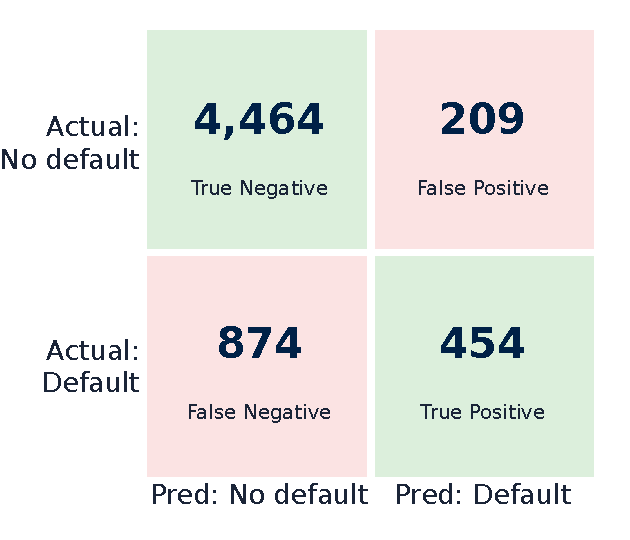
\includegraphics[width=0.9\linewidth]{fig_confusion.pdf}
    \column{0.34\textwidth}
      \centering
      {\footnotesize\textbf{Accuracy in context}}\\[0.1cm]
      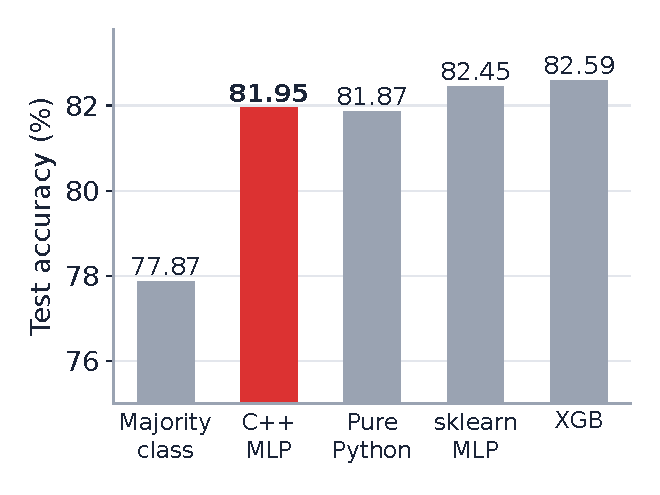
\includegraphics[width=0.9\linewidth]{fig_accuracy.pdf}
  \end{columns}

  \vspace{0.25cm}
  \begin{alertblock}{\small Reading the numbers}
    \footnotesize
    Only \textbf{34.2\%} of real defaulters are caught (454 of 1,328); accuracy looks good mainly because 78\% of clients do not default.
    Every model, from this C++ MLP to XGBoost, lands within 81.9--82.6\%: the dataset has a low ceiling\cit{10}.
    Over 10 seeds the C++ MLP scores \textbf{81.4 $\pm$ 0.5\%}.
  \end{alertblock}
\end{frame}

% ============================================================
% 8. RESULTS 2: SPEED
% ============================================================
\begin{frame}{Results: Speed and Efficiency}
  \begin{columns}[T]
    \column{0.49\textwidth}
      \centering
      {\footnotesize\textbf{Training time per epoch}}\\[0.1cm]
      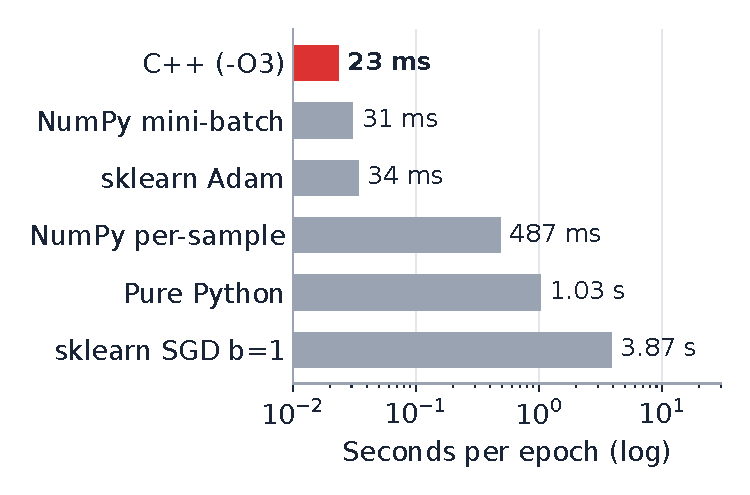
\includegraphics[width=\linewidth]{fig_train.pdf}
    \column{0.49\textwidth}
      \centering
      {\footnotesize\textbf{Single-prediction latency}}\\[0.1cm]
      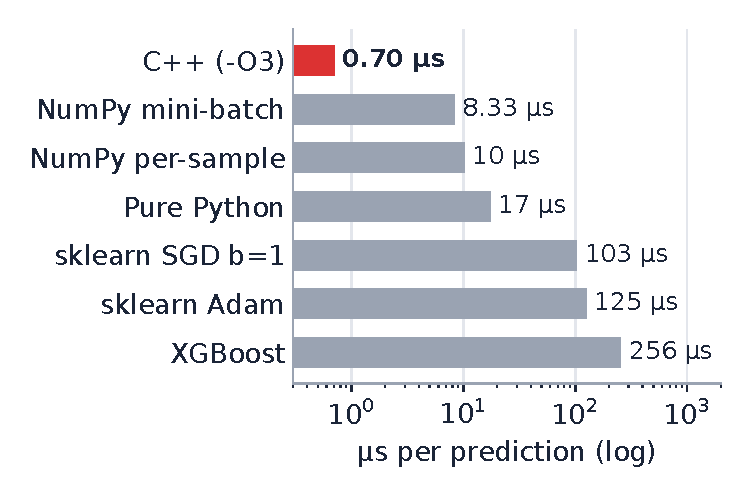
\includegraphics[width=\linewidth]{fig_latency.pdf}
  \end{columns}

  \vspace{0.1cm}
  \begin{columns}[T]
    \column{0.31\textwidth}
      \begin{block}{\scriptsize Training (80 epochs)}
\begin{eq}{1.05cm}
        \scriptsize C++ \textbf{1.87 s} vs.\ pure Python 82.6 s: \textbf{about 44$\times$ faster}
      \end{eq}
      \end{block}
    \column{0.31\textwidth}
      \begin{block}{\scriptsize Latency, per prediction}
\begin{eq}{1.05cm}
        \scriptsize C++ \textbf{0.70\,\textmu s} vs.\ Python 17.4\,\textmu s: \textbf{about 25$\times$ lower}
      \end{eq}
      \end{block}
    \column{0.31\textwidth}
      \begin{alertblock}{\scriptsize Vs.\ libraries (one call)}
\begin{eq}{1.05cm}
        \scriptsize sklearn\cit{8} / XGBoost\cit{7} take 103--256\,\textmu s per call: \textbf{about 145--365$\times$ higher}
      \end{eq}
      \end{alertblock}
  \end{columns}
\end{frame}

% ============================================================
% 9. RESULTS 3: FULL COMPARISON
% ============================================================
\begin{frame}{Results: C++ vs.\ Python vs.\ Libraries}
  \centering
  \footnotesize
  \setlength{\tabcolsep}{5pt}
  \begin{tabular}{@{}lrrrrrr@{}}
    \toprule
    \textbf{Implementation} & \textbf{Train} & \textbf{Per pred.} & \textbf{Batch} & \textbf{Acc.} & \textbf{F1} & \textbf{AUC} \\
     & {\scriptsize(80 ep.)} & {\scriptsize(\textmu s)} & {\scriptsize(\textmu s/row)} & {\scriptsize(\%)} & {\scriptsize(\%)} & \\
    \midrule
    \rowcolor{accent!12}
    \textbf{C++ MLP (this work)}  & \textbf{1.87 s} & \textbf{0.70} & 0.70 & 81.95 & 45.6 & 0.771 \\
    Pure Python (no libraries)    & 82.6 s          & 17.4          & 17.4 & 81.87 & 45.2 & -- \\
    NumPy\cit{9}, per-sample SGD     & 38.9 s          & 10.2          & 0.53 & 81.89 & 45.3 & 0.771 \\
    NumPy, mini-batch (32)        & 2.45 s          & 8.3           & 0.06 & 82.52 & 48.8 & 0.771 \\
    scikit-learn\cit{8} MLP, Adam    & 2.71 s          & 125.2         & 0.13 & 82.45 & 49.7 & 0.777 \\
    scikit-learn MLP, SGD b=1     & 3.87 s/ep.$^{\dagger}$ & 102.7  & 0.14 & 82.47 & 44.8 & 0.764 \\
    XGBoost\cit{7} (200 trees)       & 0.75 s          & 255.8         & 1.81 & 82.59 & 49.6 & 0.787 \\
    \bottomrule
  \end{tabular}

  \vspace{0.15cm}
  \begin{columns}[T]
    \column{0.48\textwidth}
      \begin{block}{\scriptsize What the table says}
\begin{eq}{2.0cm}
        \scriptsize
        \begin{itemize}
          \item Libraries match C++ at \textbf{training} with mini-batches
          \item C++ wins \textbf{one-at-a-time} prediction (call overhead dominates)
          \item SIMD adds only $\approx$6\%; the speed comes mostly from \textbf{avoiding overhead}
        \end{itemize}
      \end{eq}
      \end{block}
    \column{0.48\textwidth}
      \begin{alertblock}{\scriptsize Caveats}
\begin{eq}{2.0cm}
        \scriptsize
        $^{\dagger}$5 epochs only. All rows share one split; C++, Python and NumPy also share initial weights
        and shuffles (C++ in \texttt{double} matches Python exactly). Times: medians, noisy 2-vCPU machine.
      \end{eq}
      \end{alertblock}
  \end{columns}
\end{frame}


% ============================================================
% 10a. RESULTS 4: LEARNING BEHAVIOUR + ROC
% ============================================================
\begin{frame}{Results: Learning Behaviour and ROC}
  \begin{columns}[T]
    \column{0.49\textwidth}
      \centering
      {\footnotesize\textbf{Training curves (C++ MLP, 80 epochs)}}\\[0.1cm]
      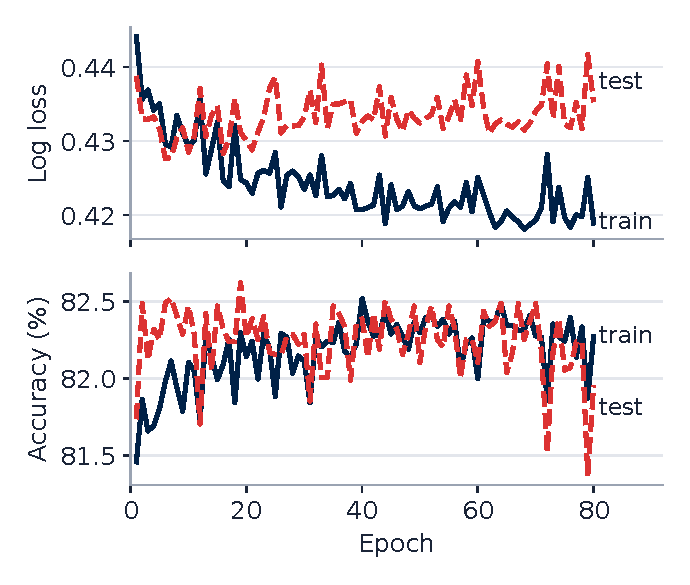
\includegraphics[height=4.5cm]{fig_curves.pdf}
    \column{0.49\textwidth}
      \centering
      {\footnotesize\textbf{ROC curves, held-out test set}}\\[0.1cm]
      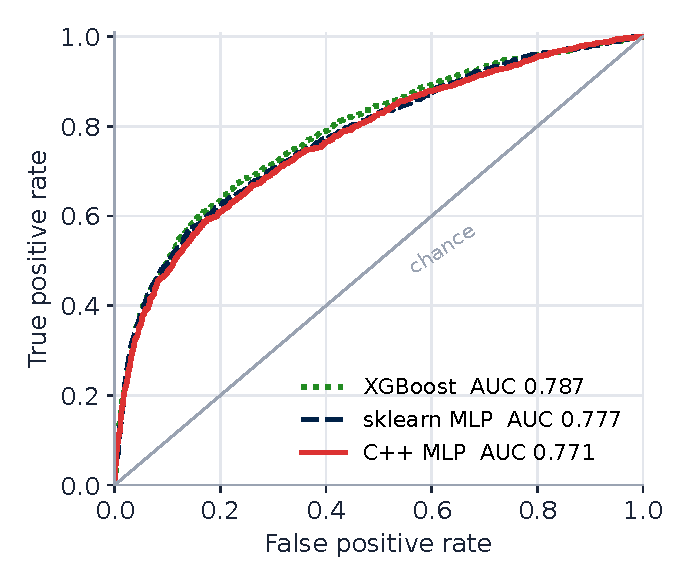
\includegraphics[height=4.5cm]{fig_roc.pdf}
  \end{columns}

  \vspace{0.1cm}
  \begin{columns}[T]
    \column{0.48\textwidth}
      \begin{block}{\scriptsize Training behaviour}
\begin{eq}{1.05cm}
        \scriptsize Training loss falls from 0.444 to 0.419, but test loss stays flat at about 0.43--0.44:
        little is gained after the first few epochs.
      \end{eq}
      \end{block}
    \column{0.48\textwidth}
      \begin{alertblock}{\scriptsize Ranking quality (AUC)}
\begin{eq}{1.05cm}
        \scriptsize C++ \textbf{0.771}, sklearn 0.777, XGBoost 0.787. The curves nearly overlap; AUC does not depend on the 0.5 threshold.
      \end{eq}
      \end{alertblock}
  \end{columns}
\end{frame}

% ============================================================
% 10b. RESULTS 5: THRESHOLD + SEEDS
% ============================================================
\begin{frame}{Results: Decision Threshold and Robustness}
  \begin{columns}[T]
    \column{0.49\textwidth}
      \centering
      {\footnotesize\textbf{Metrics vs.\ decision threshold (C++ MLP)}}\\[0.1cm]
      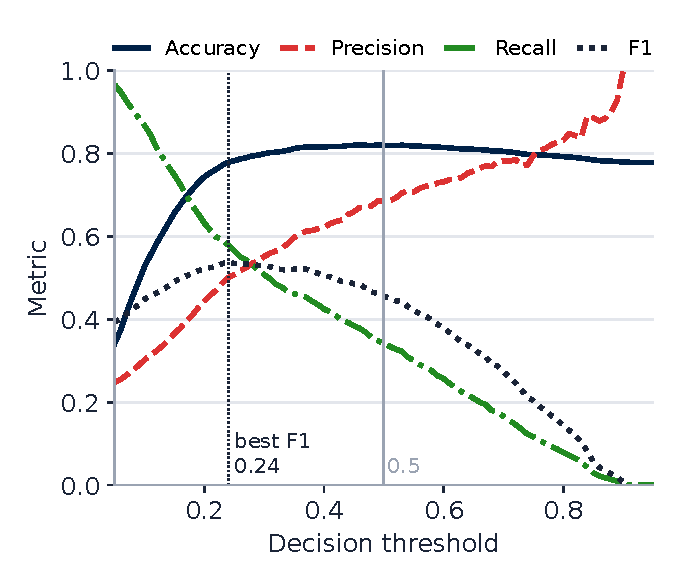
\includegraphics[height=4.5cm]{fig_threshold.pdf}
    \column{0.49\textwidth}
      \centering
      {\footnotesize\textbf{Same 10 seeds for every model}}\\[0.1cm]
      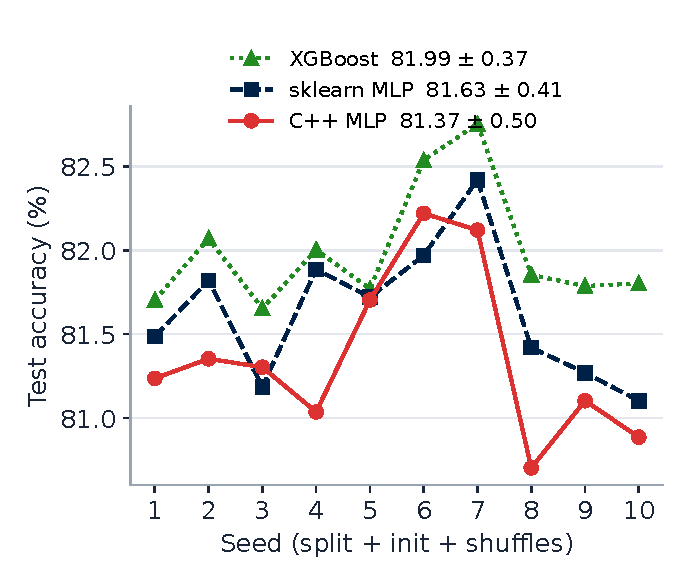
\includegraphics[height=4.5cm]{fig_seeds.pdf}
  \end{columns}

  \vspace{0.1cm}
  \begin{columns}[T]
    \column{0.48\textwidth}
      \begin{block}{\scriptsize Threshold matters more than the model}
\begin{eq}{1.05cm}
        \scriptsize At 0.24 the F1 peaks at \textbf{53.7\%} with recall \textbf{57.9\%} (34.2\% at 0.5), at 77.9\% accuracy.
        Lenders should pick the threshold from loss costs.
      \end{eq}
      \end{block}
    \column{0.48\textwidth}
      \begin{alertblock}{\scriptsize Paired comparison (10 seeds)}
\begin{eq}{1.05cm}
        \scriptsize XGBoost beats the C++ MLP on \textbf{10 of 10} seeds ($+$0.63 pt); sklearn MLP on 8 of 10 ($+$0.26 pt).
      \end{eq}
      \end{alertblock}
  \end{columns}
\end{frame}

% ============================================================
% 10. APPLICATION
% ============================================================
\begin{frame}{Applications: Quant Finance and Low Latency}
  \begin{columns}[T]
    \column{0.52\textwidth}
      \begin{block}{Where microseconds matter}
        \footnotesize
        \begin{itemize}
          \item \textbf{Pre-trade / counterparty credit checks} inside order-flow latency budgets\cit{11}
          \item \textbf{Card authorization:} score each transaction's account risk in real time\cit{6}
          \item \textbf{Stress testing:} re-score a portfolio under thousands of scenarios
          \item \textbf{Expected loss:} the model supplies the PD in
                $\mathrm{EL} = \mathrm{PD}\times\mathrm{LGD}\times\mathrm{EAD}$;
                the decision threshold should come from loss costs, not 0.5
        \end{itemize}
      \end{block}
      \begin{alertblock}{\footnotesize Illustrative scale (one core, model only)}
        \scriptsize
        $10^{6}$ accounts $\times$ $10^{3}$ scenarios $=10^{9}$ scores:\\
        \textbf{C++ $\approx$ 12 min} \quad vs.\quad pure Python $\approx$ 4.8 hours
      \end{alertblock}
    \column{0.44\textwidth}
      \begin{block}{Why C++ suits this}
        \footnotesize
        \begin{itemize}
          \item \textbf{Predictable latency:} no interpreter or garbage-collector pauses, no allocation per call
          \item \textbf{Cache-resident:} 1.6\,KB of weights fit in L1 cache
          \item \textbf{Throughput:} $\approx$1.4\,M scores/s per core vs.\ $\approx$57\,k/s in Python
          \item \textbf{Deployable:} no runtime dependencies
        \end{itemize}
      \end{block}
      \begin{block}{\footnotesize Limits}
        \scriptsize
        Latency shown is \textbf{model-only}; real systems add feature retrieval, network and risk checks.
        Regulated lenders also need explainable, validated models.
      \end{block}
  \end{columns}
\end{frame}

% ============================================================
% 11. REFERENCES (IEEE)
% ============================================================
\begin{frame}{References}
  \fontsize{6.8}{8.2}\selectfont
  \setlength{\parskip}{2pt}
  \refitem{1}{I.-C. Yeh and C.-H. Lien, ``The comparisons of data mining techniques for the predictive accuracy of probability of default of credit card clients,'' \textit{Expert Syst. Appl.}, vol. 36, no. 2, pp. 2473--2480, 2009.}
  \refitem{2}{I.-C. Yeh, ``Default of credit card clients,'' UCI Machine Learning Repository, 2016. [Online]. Available: https://archive.ics.uci.edu/dataset/350}
  \refitem{3}{D. E. Rumelhart, G. E. Hinton, and R. J. Williams, ``Learning representations by back-propagating errors,'' \textit{Nature}, vol. 323, pp. 533--536, 1986.}
  \refitem{4}{Y. LeCun, L. Bottou, G. B. Orr, and K.-R. M\"{u}ller, ``Efficient BackProp,'' in \textit{Neural Networks: Tricks of the Trade}. Berlin, Germany: Springer, 1998, pp. 9--50.}
  \refitem{5}{K. He, X. Zhang, S. Ren, and J. Sun, ``Delving deep into rectifiers: Surpassing human-level performance on ImageNet classification,'' in \textit{Proc. IEEE Int. Conf. Comput. Vis. (ICCV)}, 2015, pp. 1026--1034.}
  \refitem{6}{A. E. Khandani, A. J. Kim, and A. W. Lo, ``Consumer credit-risk models via machine-learning algorithms,'' \textit{J. Banking Finance}, vol. 34, no. 11, pp. 2767--2787, 2010.}
  \refitem{7}{T. Chen and C. Guestrin, ``XGBoost: A scalable tree boosting system,'' in \textit{Proc. 22nd ACM SIGKDD Int. Conf. Knowl. Discovery Data Mining}, 2016, pp. 785--794.}
  \refitem{8}{F. Pedregosa \textit{et al.}, ``Scikit-learn: Machine learning in Python,'' \textit{J. Mach. Learn. Res.}, vol. 12, pp. 2825--2830, 2011.}
  \refitem{9}{C. R. Harris \textit{et al.}, ``Array programming with NumPy,'' \textit{Nature}, vol. 585, pp. 357--362, 2020.}
  \refitem{10}{L. Grinsztajn, E. Oyallon, and G. Varoquaux, ``Why do tree-based models still outperform deep learning on typical tabular data?'' in \textit{Proc. Adv. Neural Inf. Process. Syst. (NeurIPS), Datasets Benchmarks Track}, vol. 35, 2022.}
  \refitem{11}{I. Aldridge, \textit{High-Frequency Trading: A Practical Guide to Algorithmic Strategies and Trading Systems}, 2nd ed. Hoboken, NJ, USA: Wiley, 2013.}
\end{frame}

% ============================================================
% 13. THANK YOU
% ============================================================
{
\setbeamercolor{background canvas}{bg=primary}
\begin{frame}[plain]
  \centering
  \vspace{1.5cm}
  {\color{accent}\rule{1.2cm}{1.2mm}}\\[0.4cm]
  {\color{white}\Large\textbf{Thank You}}\\[0.4cm]
  {\color{white!70}\normalsize Questions \& Discussion}\\[0.5cm]
  {\color{white!25}\rule{0.5\textwidth}{0.5pt}}\\[0.4cm]
  {\color{white!60}\small
    Arya H. Raval | ID: 25EC415\\[0.1cm]
    204ES: Object Oriented Programming\\
    Electronics \& Communication Engineering \\
    Birla Vishvakarma Mahavidyalaya
  }
\end{frame}
}

% ============================================================
% APPENDIX
% ============================================================
\appendix
\section{Appendix}
\setbeamertemplate{footline}{%
  \vbox{\hbox to\paperwidth{\hskip6mm{\color{primary!55}\fontsize{6.5}{8}\selectfont\bfseries ARYA H. RAVAL\ \ $\cdot$\ \ 25EC415\ \ $\cdot$\ \ 204ES: OBJECT ORIENTED PROGRAMMING}\hfill
    {\color{primary!55}\fontsize{6.5}{8}\selectfont\bfseries APPENDIX}\hskip6mm}\vskip0.5mm
   {\color{primary!35}\rule{\paperwidth}{0.6mm}}\vskip-0.2mm}}

{
\setbeamercolor{background canvas}{bg=primary}
\begin{frame}[plain]
  \centering
  \vspace{2.2cm}
  {\color{accent}\rule{1.2cm}{1.2mm}}\\[0.4cm]
  {\color{white}\Large\textbf{Appendix}}\\[0.3cm]
  {\color{white!70}\small A. The \texttt{FastMLP} class \ $\cdot$\ B. Backpropagation \ $\cdot$\ C. File management \ $\cdot$\ D. Metrics and training loop}
\end{frame}
}

% ============================================================
% 6c. CODE: THE CLASS
% ============================================================
\begin{frame}[fragile]{Appendix A: The \texttt{FastMLP} Class}
  \begin{columns}[T]
    \column{0.60\textwidth}
\begin{lstlisting}[style=cpp]
class FastMLP {
    int nIn, nH;                 // layer sizes
    vector<float> W1, b1, W2;    // weights, biases
    float b2, lr;                // output bias, step
    mutable vector<float> h_buf; // scratch space
    vector<float> dh_buf, dW2_buf;

public:
    FastMLP(int in, int hidden, float rate = 0.01f)
        : nIn(in), nH(hidden), W1(hidden * in),
          b1(hidden, 0.0f), W2(hidden), b2(0.0f),
          lr(rate), h_buf(hidden) {
        mt19937 gen(42);                 // fixed seed
        normal_distribution<float>
            d1(0.0f, sqrt(2.0f / in));   // He init
        for (auto &w : W1) w = d1(gen);
        // W2 is initialised the same way
    }
    float forward(const float* x,
                  vector<float>& h) const;
    float predict(const vector<float>& x) const;
    void  trainOne(const Sample& s);
};
\end{lstlisting}
      {\tiny abridged: a few buffer members and the W2 initialisation are omitted.}
    \column{0.37\textwidth}
      \begin{block}{\small What to notice}
        \scriptsize
        \begin{itemize}
          \item \textbf{Encapsulation:} data is private; only three public methods
          \item \textbf{Constructor:} the \emph{init list} sizes every array before the body runs, so the object is never half-built
          \item \textbf{He init:} $\mathcal{N}(0,2/n_{\text{in}})$ keeps signals at a sensible scale\cit{5}
          \item \textbf{\texttt{mutable}:} lets the \texttt{const} method \texttt{predict()} reuse \texttt{h\_buf} with no allocation
        \end{itemize}
      \end{block}
      \begin{block}{\small Creating the object}
\begin{lstlisting}[style=cpp]
FastMLP net(23, 16, 0.01f);
net.trainOne(sample);
float p = net.predict(x);
\end{lstlisting}
      \end{block}
  \end{columns}
\end{frame}

% ============================================================
% 6e. CODE: BACKPROPAGATION
% ============================================================
\begin{frame}[fragile]{Appendix B: Learning by Backpropagation}
  \begin{columns}[T]
    \column{0.56\textwidth}
\begin{lstlisting}[style=cpp]
void trainOne(const Sample& s) {
    float p  = forward(s.x.data(), h_buf);
    float dz = p - s.y;              // output error

    for (int j = 0; j < nH; ++j) {
        dW2_buf[j] = dz * h_buf[j];
        dh_buf[j]  = dz * W2[j]
                   * (1.0f - h_buf[j] * h_buf[j]);
    }
    for (int j = 0; j < nH; ++j) {   // gradient step
        float dh = dh_buf[j];
        float* w_row = &W1[j * nIn];
        for (int i = 0; i < nIn; ++i)
            w_row[i] -= lr * dh * s.x[i];
        b1[j] -= lr * dh;
        W2[j] -= lr * dW2_buf[j];
    }
    b2 -= lr * dz;
}
\end{lstlisting}
    \column{0.41\textwidth}
      \begin{block}{\small The maths, line by line\cit{3,4}}
        \scriptsize
        Loss for one client: $L=-[\,y\ln p+(1-y)\ln(1-p)\,]$
        \begin{align*}
          dz &= \tfrac{\partial L}{\partial z} = p - y\\
          \tfrac{\partial L}{\partial w_j} &= dz\,h_j\\
          \delta_j &= dz\,w_j\,(1-h_j^{2})\\
          \tfrac{\partial L}{\partial W_{ji}} &= \delta_j\,x_i\\
          \theta &\leftarrow \theta - \eta\,\tfrac{\partial L}{\partial \theta}
        \end{align*}
      \end{block}
  \end{columns}
  \vspace{0.05cm}
  {\scriptsize\textbf{Reading it:} $dz$ says how wrong the guess was; $(1-h_j^2)$ is the slope of $\tanh$; each weight moves a small step $\eta=0.01$ against its share of the error. This runs once per client, 80 epochs.}
\end{frame}

% ============================================================
% 6f. CODE: FILE HANDLING AND DATA
% ============================================================
\begin{frame}[fragile]{Appendix C: File Management and Data Preparation}
  \begin{columns}[T]
    \column{0.575\textwidth}
\begin{lstlisting}[style=cpp]
vector<Sample> loadCSV(const string& file) {
    ifstream f(file);                  // open
    if (!f) { cerr << "Cannot open " << file;
              exit(1); }               // check
    string line; getline(f, line);     // skip header
    vector<Sample> data;
    while (getline(f, line)) {
        auto c = split(line);          // split on ','
        if (c.size() < 25) continue;   // bad row
        Sample s;
        for (int i = 1; i <= 23; ++i)  // col 0 = ID
            s.x.push_back(stof(c[i])); // text -> float
        s.y = stoi(c[24]);             // label
        data.push_back(s);
    }
    return data;       // f closes automatically
}

vector<string> split(const string& line) {
    vector<string> a; string s;
    stringstream ss(line);
    while (getline(ss, s, ',')) a.push_back(s);
    return a;
}
\end{lstlisting}
    \column{0.40\textwidth}
      \begin{block}{\small File handling}
        \scriptsize
        \begin{itemize}
          \item \texttt{ifstream} opens the file; \texttt{if (!f)} stops cleanly if it is missing
          \item \texttt{getline} reads one row at a time, so the whole file is never held as text
          \item \texttt{stringstream} cuts a row into 25 fields
          \item The file closes itself when \texttt{f} leaves scope (RAII)
        \end{itemize}
      \end{block}
      \begin{block}{\small Standardize, training statistics only\cit{4}}
        \scriptsize
        \[ x'_{j} = \frac{x_j-\mu_j}{\sigma_j} \]
\begin{lstlisting}[style=cpp]
s.x[j] = (s.x[j] - mu[j]) / sd[j];
\end{lstlisting}
        $\mu_j,\sigma_j$ come from the 80\% training split and are applied unchanged to the test split.
      \end{block}
  \end{columns}
\end{frame}

% ============================================================
% 6g. CODE: METRICS AND TRAINING LOOP
% ============================================================
\begin{frame}[fragile]{Appendix D: Metrics Struct and the Training Loop}
  \begin{columns}[T]
    \column{0.55\textwidth}
\begin{lstlisting}[style=cpp]
struct Metrics {
    int tp=0, tn=0, fp=0, fn=0;
    float accuracy() const
        { return float(tp+tn) / (tp+tn+fp+fn); }
    float precision() const
        { return tp+fp ? float(tp)/(tp+fp) : 0; }
    float recall() const
        { return tp+fn ? float(tp)/(tp+fn) : 0; }
    float f1() const {
        float p = precision(), r = recall();
        return p+r ? 2*p*r/(p+r) : 0;
    }
};
\end{lstlisting}
      \vspace{0.15cm}
\begin{lstlisting}[style=cpp]
FastMLP net(23, 16, 0.01f);        // the object
for (int e = 1; e <= 80; ++e) {    // epochs
    shuffle(train.begin(), train.end(), rng);
    for (const auto& s : train)
        net.trainOne(s);           // one SGD step
}
\end{lstlisting}
    \column{0.42\textwidth}
      \begin{block}{\small A struct with behaviour}
        \scriptsize
        \texttt{Metrics} keeps its four counters and the formulas that use them together. Each method is \texttt{const}: reading a score never changes the counts.
        \[ P=\tfrac{TP}{TP+FP},\; R=\tfrac{TP}{TP+FN},\; F_1=\tfrac{2PR}{P+R} \]
      \end{block}
      \begin{block}{\small The training loop}
        \scriptsize
        \begin{itemize}
          \item Shuffle every epoch so the model does not learn the row order
          \item \texttt{const auto\&} avoids copying each \texttt{Sample}
          \item \texttt{evaluate(net, test)} fills a \texttt{Metrics} object by comparing $\hat y$ with $y$
        \end{itemize}
      \end{block}
  \end{columns}
\end{frame}

\end{document}
